\documentclass[11pt,twocolumn]{article}
\usepackage[margin=0.72in]{geometry}
\usepackage{amsmath,amssymb,amsthm}
\usepackage{booktabs}
\usepackage{graphicx}
\usepackage{hyperref}
\usepackage{xcolor}
\usepackage{enumitem}

\hypersetup{
  colorlinks=true,
  linkcolor=blue!60!black,
  citecolor=green!45!black,
  urlcolor=blue!65!black
}

\newtheorem{proposition}{Proposition}

\newcommand{\ZZ}{\mathbb{Z}}
\newcommand{\QQ}{\mathbb{Q}}
\newcommand{\RR}{\mathbb{R}}

\title{\textbf{Machine-Checked Exact-Rational Checkpoint Rounding, Dual-Price Markov, and Goods/Chores $(1 \mp \varepsilon)$-MMS Allocation Certificates}}
\author{Lluis Eriksson\thanks{Independent researcher; manuscript prepared with transparent AI assistance via Google Antigravity. Source code, Lean~4 proofs, and exact certificates: \url{https://github.com/lluiseriksson/asymptotic-mms-allocation-certificates}.}}
\date{November 25, 2026}

\begin{document}
\sloppy
\maketitle

\begin{abstract}
Zehan Lin, Shengxin Liu, Biaoshuai Tao, Xiaowei Wu, and Yuhao Zhang (\texttt{arXiv:2611.33052}, November 24, 2026) resolved the asymptotic maximin share (MMS) conjecture of Feige and Grinberg for additive fair division: for every $\varepsilon > 0$ and all sufficiently large $n \ge n_0(\varepsilon)$, every instance with $n$ agents admits a $(1 - \varepsilon)$-MMS allocation for indivisible goods and a $(1 + \varepsilon)$-MMS allocation for indivisible chores, computable in randomized polynomial time using only ordinal bundle-comparison queries. We present a machine-checked, zero-floating-point formalization and exact-$\QQ$ certificate auditor for the deterministic LP-rounding, deadline-slot, Abel-summation, dual-price Markov, and exact-MMS allocation core of this breakthrough. First, an 18-theorem zero-dependency Lean~4 kernel (\texttt{AsymptoticMMS.lean}, Lean~4.35.0; 0~\texttt{sorry}, 0~warnings, 0~\texttt{Classical.choice}, 2 zero-axiom theorems) formalizes Algorithm~3.1 Step~1 checkpoint counting and Lemma~3.5 support halving, terminal rounding loss $160L$, Step~2 $\lceil k/\lambda\rceil$ strict slot monotonicity and prefix reserve $|U \cap M_{[j]}| \ge (1-\lambda)j$, exact Eq.~(3.1) Abel summation by induction, Step~3 greedy bag-filling survival, Section~3.3 dual price double-summation $p(M) = \sum_j j\alpha_j$, Definition~3.7 Markov reserved-agent decay $|N_r| L^2 < 1536 n$, reduced-MMS segment counts, dual price transfer, and the goods/chores landmark hierarchy. Second, \texttt{MMS-ASYMPTOTIC-CERT-1.0} audits four exact-$\QQ$ modes across 16 canonical certificates ($0.211$--$0.864\,\mathrm{ms}$) and rejects 60/60 live adversarial forgeries.
\end{abstract}

\section{Introduction}
Fairly allocating indivisible goods or chores under maximin share (MMS) guarantees~\cite{budish2011combinatorial} is a central problem in computational social choice. Since exact $1$-MMS allocations do not always exist~\cite{kurokawa2018fair}, a decade of work advanced constant-factor approximations from $2/3$ and $3/4$ past $3/4 + 3/3836$~\cite{akrami2024breaking} to $7/9$ for goods and from $4/3$ and $11/9$~\cite{huang2021algorithmic} to $13/11$ for chores~\cite{huang2023reduction}, while Feige and Grinberg~\cite{feige2025asymptotic} conjectured that $(1 - o(1))$-MMS allocations exist asymptotically as $n \to \infty$. Lin et al.~\cite{lin2026mms} proved this conjecture for both goods and chores via an LP-based matching-and-duality architecture resting on four exact rational pillars:
\begin{enumerate}[leftmargin=*,nosep]
  \item \emph{Checkpoint rounding \& support halving (Algorithm~3.1 Step~1, Lemmas~3.4--3.5):} Given a fractional allocation on an identical-order (IDO) normalized instance ($\sum_e v_i(e)=n$, $v_i(e)\le 1$), each round imposes at most $|F|/4$ prefix checkpoints so that $|F'| \le |F|/2$, weight loss is at most $\omega |F|$, and all prefix loads stay bounded by $\lambda j$.
  \item \emph{Deadline slot assignment \& greedy bag-filling (Steps~2--3, Eq.~(3.1), Lemma~3.6):} Assigning the $\lceil k/\lambda\rceil$-th item to the $k$-th sorted deadline guarantees $|U \cap M_{[j]}| \ge j - \lfloor \lambda j\rfloor \ge (1-\lambda)j$; Abel summation
  \begin{equation}
    v_i(U) = \sum_{j=1}^{m} |U \cap M_{[j]}| \bigl(v_i(e_j) - v_i(e_{j+1})\bigr) \ge n(1-\lambda)
    \label{eq:abel}
  \end{equation}
  then certifies enough pool value $\Delta = n(1-\lambda)$ to satisfy every unserved agent via greedy bag-filling.
  \item \emph{Small-slack dual LP prices \& Markov partition (Section~3.3, Def.~3.7, Lemma~3.8, Eq.~(3.2)):} When $\Delta < 2R = 1536 L^2$, dual variables $(\zeta_i, \alpha_j)$ define non-increasing item prices $p(e_k) = \sum_{j\ge k} \alpha_j$ with $\sum_k p(e_k) = \sum_j j\alpha_j = n$, partitioning agents into ordinary ($n(1-\zeta_i) \le L^4$) and reserved ($|N_r| L^2 < 1536 n$) sets and concentrating almost all price on the valuable prefix $M_1$.
  \item \emph{Exact $(1-\varepsilon)$-MMS goods and $(1+\varepsilon)$-MMS chores with ordinal comparisons:} Finite allocations satisfy every agent within $1\mp\varepsilon$ of exact MMS witnesses while respecting comparison-only bundle queries.
\end{enumerate}

\paragraph{Contributions and Scope.}
We mechanize and audit the deterministic algebraic, LP-rounding, Abel-summation, dual-price, and exact-MMS allocation core of~\cite{lin2026mms}. We explicitly scope our Lean~4 kernel away from the randomized exponential-size LP ellipsoid/MWU solver, the asymptotic $n \ge n_0(\varepsilon)$ Chernoff/union-bound sampling step, and the Section~5 non-additive chores reduction:
\begin{enumerate}[leftmargin=*,nosep]
  \item \textbf{Zero-dependency Lean~4 kernel (\S\ref{sec:lean}):} 18 constructive theorems in \texttt{AsymptoticMMS.lean} (Lean~4.35.0~\cite{demoura2021lean4}), 0~\texttt{sorry}, 0~warnings, 0~\texttt{Classical.choice}, and 2 zero-axiom theorems.
  \item \textbf{Pure-stdlib exact-\texorpdfstring{$\QQ$}{Q} verifier (\S\ref{sec:certifier}):} \texttt{MMS-ASYMPTOTIC-CERT-1.0}, auditing checkpoint rounding, Step~2/3 deadline and bag-filling replay with Eq.~\eqref{eq:abel}, Section~3.3 dual price certificates, and tight exact-MMS goods/chores allocations with ordinal comparison checks.
  \item \textbf{Empirical atlas \& red-team audit (\S\ref{sec:results}):} 16 canonical certificates ($0.211$--$0.864\,\mathrm{ms}$), support-halving and reserve profiles, Markov decay curves, and 60/60 rejected live adversarial forgeries.
\end{enumerate}

\section{Zero-Dependency Lean 4 Kernel}\label{sec:lean}
We formalize 18 constructive theorems in \texttt{lean/AsymptoticMMS.lean} (Lean~4.35.0, zero external dependencies), audited by \texttt{lean/AuditAxioms.lean} with 0~warnings, 0~\texttt{sorry}, 0~\texttt{Classical.choice}, and 0~\texttt{Lean.ofReduceBool} (Table~\ref{tab:lean}): 2 zero-axiom (\texttt{none}), 3 \texttt{[propext]}, and 13 \texttt{[propext, Quot.sound]}.

\begin{proposition}[Constructive Asymptotic-MMS Kernel]\label{prop:lean}
\leavevmode
\begin{enumerate}[leftmargin=*,nosep]
  \item \emph{Checkpoint rounding \& support halving (Theorems~1--4):} Lemma~3.5 halving $2|F'| \le |F|$ from $4|C| \le |F|$, $2|A| \le |F'|$, $|F'| \le |C|+|A|$; Lemma~3.4 slack absorption $w_d(\mathrm{load}+\mathrm{inc}) \le w_d\,\mathrm{cap}$ from $w_d\,\mathrm{load}+w_n A \le w_d\,\mathrm{cap}$ and $w_d\,\mathrm{inc} \le w_n A$; Lemma~3.5 threshold count $w_n(w_k+P) < 4 w_d w_k$; and terminal rounding loss $F \le 160L$ when $w_d \le 2w_n$ and $w_n F \le 80 L w_d$.
  \item \emph{Step~2/3 deadlines, Abel summation, \& bag-filling (Theorems~5--9):} Strict slot monotonicity $\lceil k/\lambda\rceil < \lceil(k+1)/\lambda\rceil$ for $\lambda \le 1$; deadline feasibility $\lceil k/\lambda\rceil \le d$; prefix reserve $(l_d-l_n)j \le l_d(j-\mathrm{used})$; inductive exact proof of Eq.~\eqref{eq:abel} (\texttt{eq31\_abel\_summation\_exact}); and bag-filling survival $\sigma < \Delta - 2rD$ whenever $\sigma < D$, $r \le R-1$, and $2RD \le \Delta$.
  \item \emph{Section~3.3 dual prices, Markov decay, \& landmarks (Theorems~10--18):} Inductive double-sum identity $\sum_k p(e_k) = \sum_j j\alpha_j$; Definition~3.7 Markov bound $|N_r|L^2 < 1536 n$; reduced-MMS segment count $(t-1)(D-\sigma) < 2D$; per-segment dual transfer $\zeta \le p(B)-p(B') \Rightarrow p(B') \le p(B)-\zeta$; exact goods ($2/3 < 3/4 < 7/9 < 39/40 < 1$) and chores ($1 < 44/43 < 13/11 < 4/3$) landmark orderings; symmetric $(1-\varepsilon)(1+\varepsilon) = 1-\varepsilon^2 < 1$; uniform LP feasibility; and strong-duality slack identity.
\end{enumerate}
\end{proposition}

\begin{table}[t]
\centering
\caption{Complete 18-theorem Lean~4.35.0 kernel in \texttt{AsymptoticMMS.lean} (0~\texttt{sorry}, 0~warnings, 0~\texttt{Classical.choice}).}
\label{tab:lean}
\resizebox{\columnwidth}{!}{%
\begin{tabular}{@{}rll@{}}
\toprule
\# & Lean~4 Theorem Identifier & Axiom Footprint \\
\midrule
1 & \texttt{support\_halving\_lemma35} & \texttt{[propext, Quot.sound]} \\
2 & \texttt{prefix\_load\_slack\_absorption} & \texttt{[propext, Quot.sound]} \\
3 & \texttt{checkpoint\_threshold\_count\_bound} & \texttt{[propext, Quot.sound]} \\
4 & \texttt{terminal\_rounding\_loss\_160L} & \texttt{[propext, Quot.sound]} \\
5 & \texttt{step2\_assigned\_slots\_strictly\_increasing} & \texttt{[propext, Quot.sound]} \\
6 & \texttt{step2\_deadline\_feasibility} & \texttt{[propext, Quot.sound]} \\
7 & \texttt{step2\_unassigned\_prefix\_reserve} & \texttt{[propext, Quot.sound]} \\
8 & \texttt{eq31\_abel\_summation\_exact} & \texttt{[propext, Quot.sound]} \\
9 & \texttt{step3\_bag\_filling\_survival} & \texttt{[propext, Quot.sound]} \\
10 & \texttt{dual\_price\_double\_sum\_exact} & \texttt{[propext, Quot.sound]} \\
11 & \texttt{reserved\_agent\_markov\_bound} & \texttt{[propext]} \\
12 & \texttt{reduced\_mms\_segment\_count\_bound} & \texttt{[propext, Quot.sound]} \\
13 & \texttt{dual\_price\_transfer\_segment} & \texttt{[propext, Quot.sound]} \\
14 & \texttt{mms\_goods\_landmark\_ordering} & \texttt{none} \\
15 & \texttt{mms\_chores\_landmark\_ordering} & \texttt{none} \\
16 & \texttt{goods\_chores\_symmetric\_epsilon} & \texttt{[propext, Quot.sound]} \\
17 & \texttt{uniform\_mms\_fractional\_feasibility} & \texttt{[propext]} \\
18 & \texttt{strong\_duality\_slack\_identity} & \texttt{[propext]} \\
\bottomrule
\end{tabular}}
\end{table}

\section{Exact-\texorpdfstring{$\QQ$}{Q} Verifier Architecture}\label{sec:certifier}
\texttt{MMS-ASYMPTOTIC-CERT-1.0} (\texttt{src/mms\_certifier.py}) is a pure-stdlib zero-float verifier with strict JSON typing, canonical reduced rationals, and uniform 2048-bit / 1024-char DoS bounds across four modes:
\begin{enumerate}[leftmargin=*,nosep]
  \item \textbf{Mode~1 (\texttt{checkpoint\_rounding\_\allowbreak prefix\_cert}):} Audits IDO normalized valuations, capped candidate lists ($\le 256$ per agent), bundle thresholds $\ge \sigma$, integrality/support preservation, Lemma~3.5 halving $2|F'| \le |F|$ and $1 \le |C| \le |F|/4$, weight loss $\le \omega |F|$, strictly increasing checkpoints with non-increasing checkpoint loads, and all prefix loads $\le \lambda j$.
  \item \textbf{Mode~2 (\texttt{deadline\_slot\_and\_\allowbreak bagfill\_cert}):} Independently replays Step~2 $\lceil k/\lambda\rceil$ deadline assignment (including strict leftward slot reassignment), audits $|U \cap M_{[j]}| \ge j - \lfloor\lambda j\rfloor$ and exact Eq.~\eqref{eq:abel} Abel summation ($\ge \Delta$), replays Step~3 greedy bag-filling, and certifies global disjointness and $\ge \sigma$ for all $n$ agents.
  \item \textbf{Mode~3 (\texttt{small\_slack\_dual\_\allowbreak price\_cert}):} Verifies explicit unit-value MMS partitions $P_i$, bounded duals $0 \le \zeta_i \le 1$, exact dual prices $p(e_k) = \sum_{j\ge k}\alpha_j$ with $\sum_k p(e_k) = \sum_j j\alpha_j = n$, strong duality $\sum_i \zeta_i = n\lambda$, all reduced-MMS constraints $p(B\setminus B') \ge \zeta_i$ and Eq.~(3.2), the Markov bound $|N_r|\tau \le n\Delta$, and the IDO valuable prefix $M_1$.
  \item \textbf{Mode~4 (\texttt{goods\_and\_chores\_mms\_\allowbreak allocation\_cert}):} Prevents witness-weakening forgeries by certifying exact tight MMS benchmarks ($\min_k v_i(W_k) = \bar{v}_i$ for goods; $\max_k c_i(W_k) = \max(\bar{c}_i, \max_e c_i(e))$ for chores), verifies $(1-\varepsilon)$-MMS goods or $(1+\varepsilon)$-MMS chores ratios, and audits every ordinal bundle-comparison query.
\end{enumerate}

\section{Empirical Atlas and Red-Team Audit}\label{sec:results}
Running \texttt{scripts/run\_all\_experiments.py} produces 16 canonical certificates (4 per mode) and four exact-$\QQ$ studies, audited end-to-end by \texttt{scripts/verify\_all.py} with SHA-256 verification across all 41 tracked artifacts.

\begin{figure}[t]
  \centering
  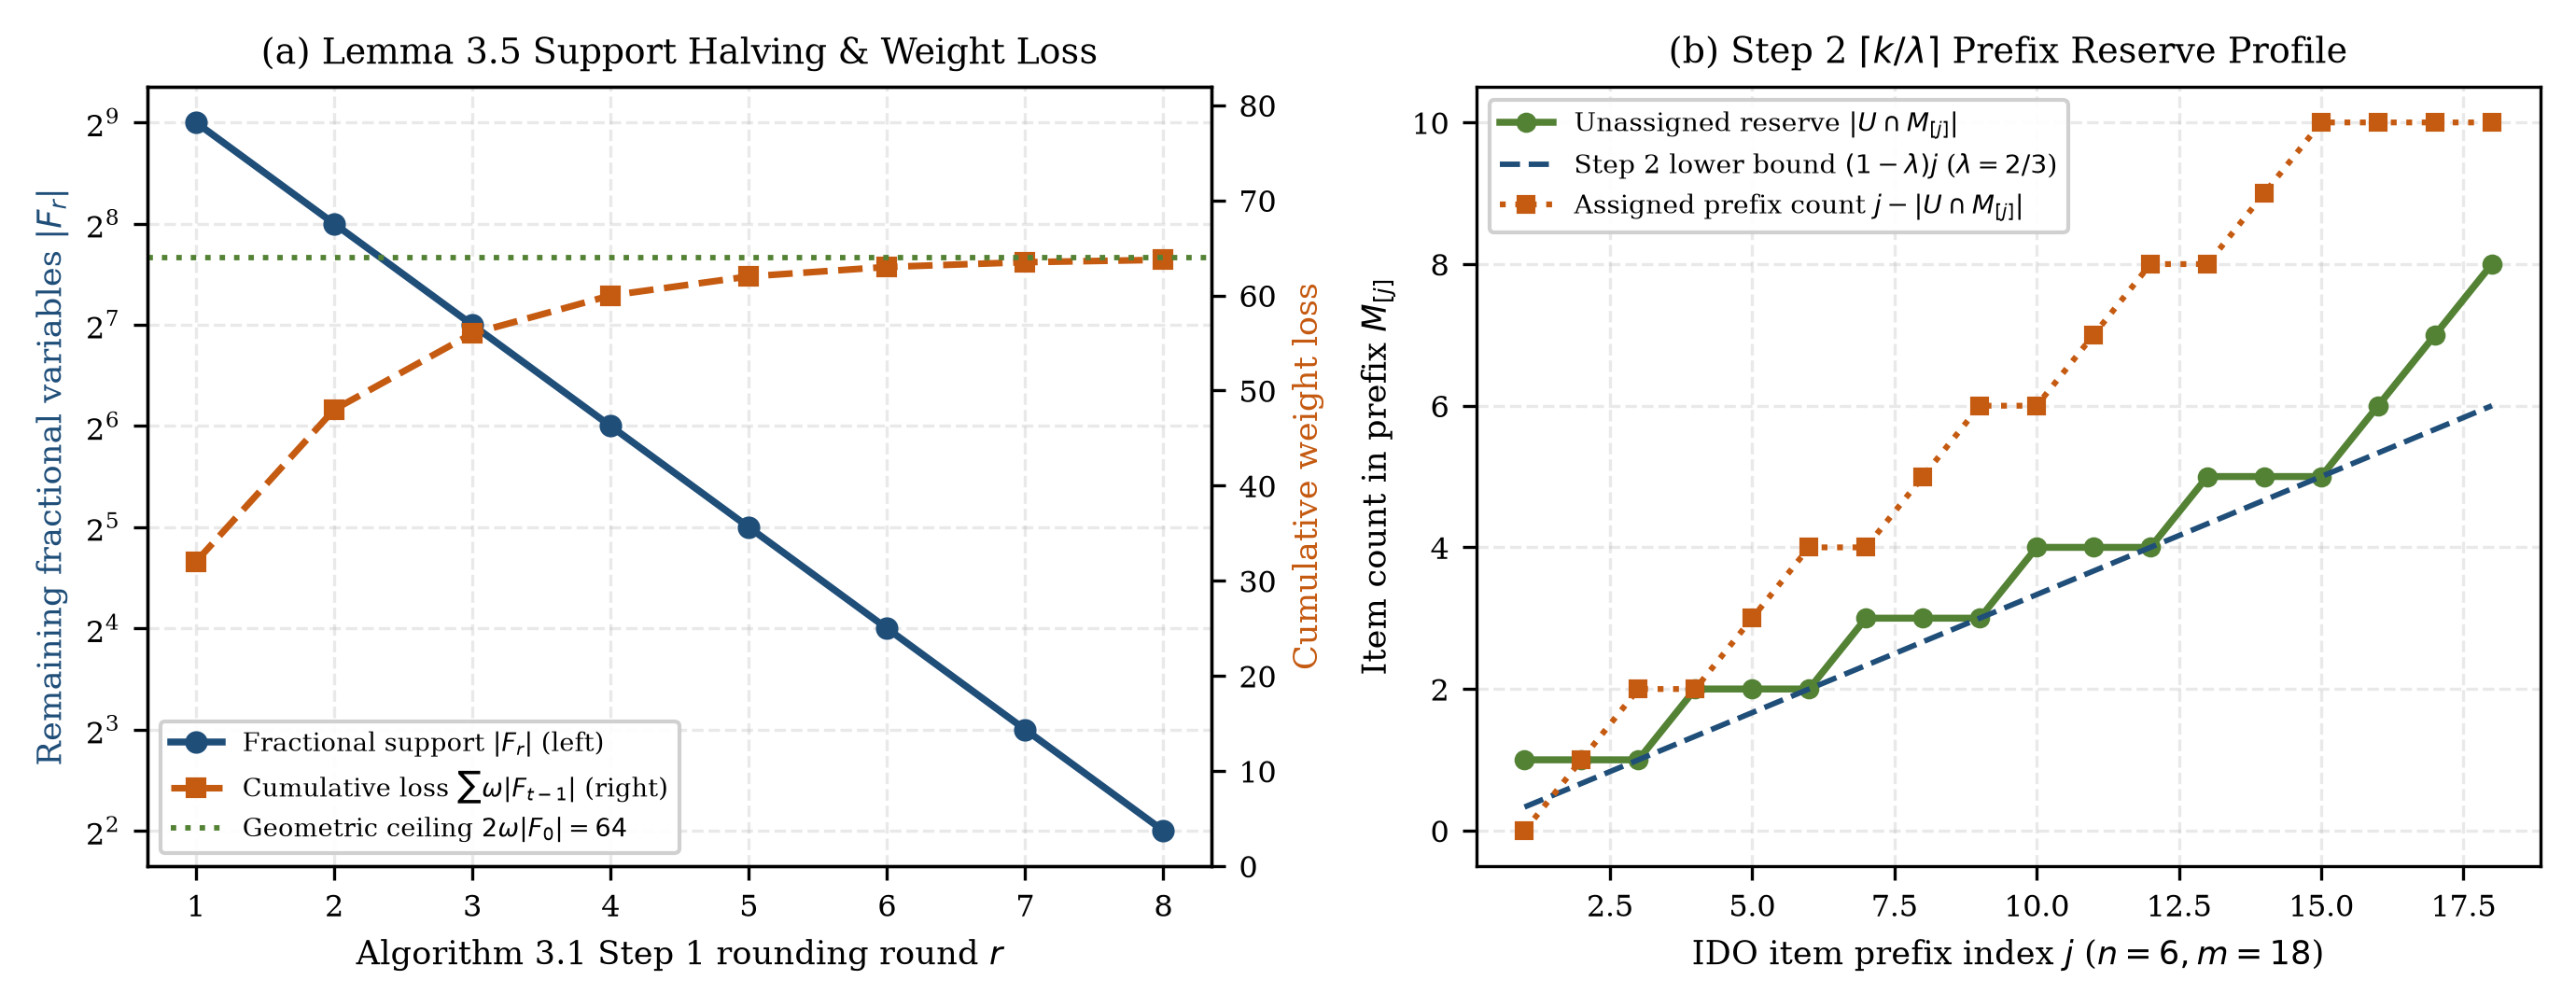
\includegraphics[width=\columnwidth]{../figures/fig1_rounding_and_reserve.png}
  \caption{(a) Algorithm~3.1 Step~1 support halving ($|F_0|=1024 \to |F_8|=4$, $\omega=1/32$) with cumulative weight loss saturating at $63.75 < 2\omega |F_0| = 64$. (b) Exact Step~2 prefix reserve $|U \cap M_{[j]}|$ vs.\ lower bound $(1-\lambda)j$ across $j=1\dots 18$ for $n=6, m=18, \lambda=2/3$.}
  \label{fig:rounding}
\end{figure}

\paragraph{Support Halving and Step~2 Prefix Reserve (Fig.~\ref{fig:rounding}).}
Starting from $|F_0| = 1024$ fractional variables with $\omega = 1/32$, eight Lemma~3.5 rounding steps halve $|F_r|$ geometrically from $512$ to $4$ while total weight loss converges to $63.75$, staying strictly beneath the geometric ceiling $2\omega |F_0| = 64$. On the $n=6, m=18, \lambda=2/3$ Mode~2 instance, Step~2's $\lceil k/\lambda\rceil$ slot schedule maintains $|U \cap M_{[j]}| \ge (1-\lambda)j$ at every prefix $j=1\dots 18$ (reaching $8 \ge 6$ at $j=18$), yielding exact Eq.~\eqref{eq:abel} pool value $\min_i v_i(U) = 12/5 > \Delta = 2$ and Step~3 bag-filling value $\min_i v_i(X_i) = 17/20 \ge \sigma = 3/4$.

\begin{figure}[t]
  \centering
  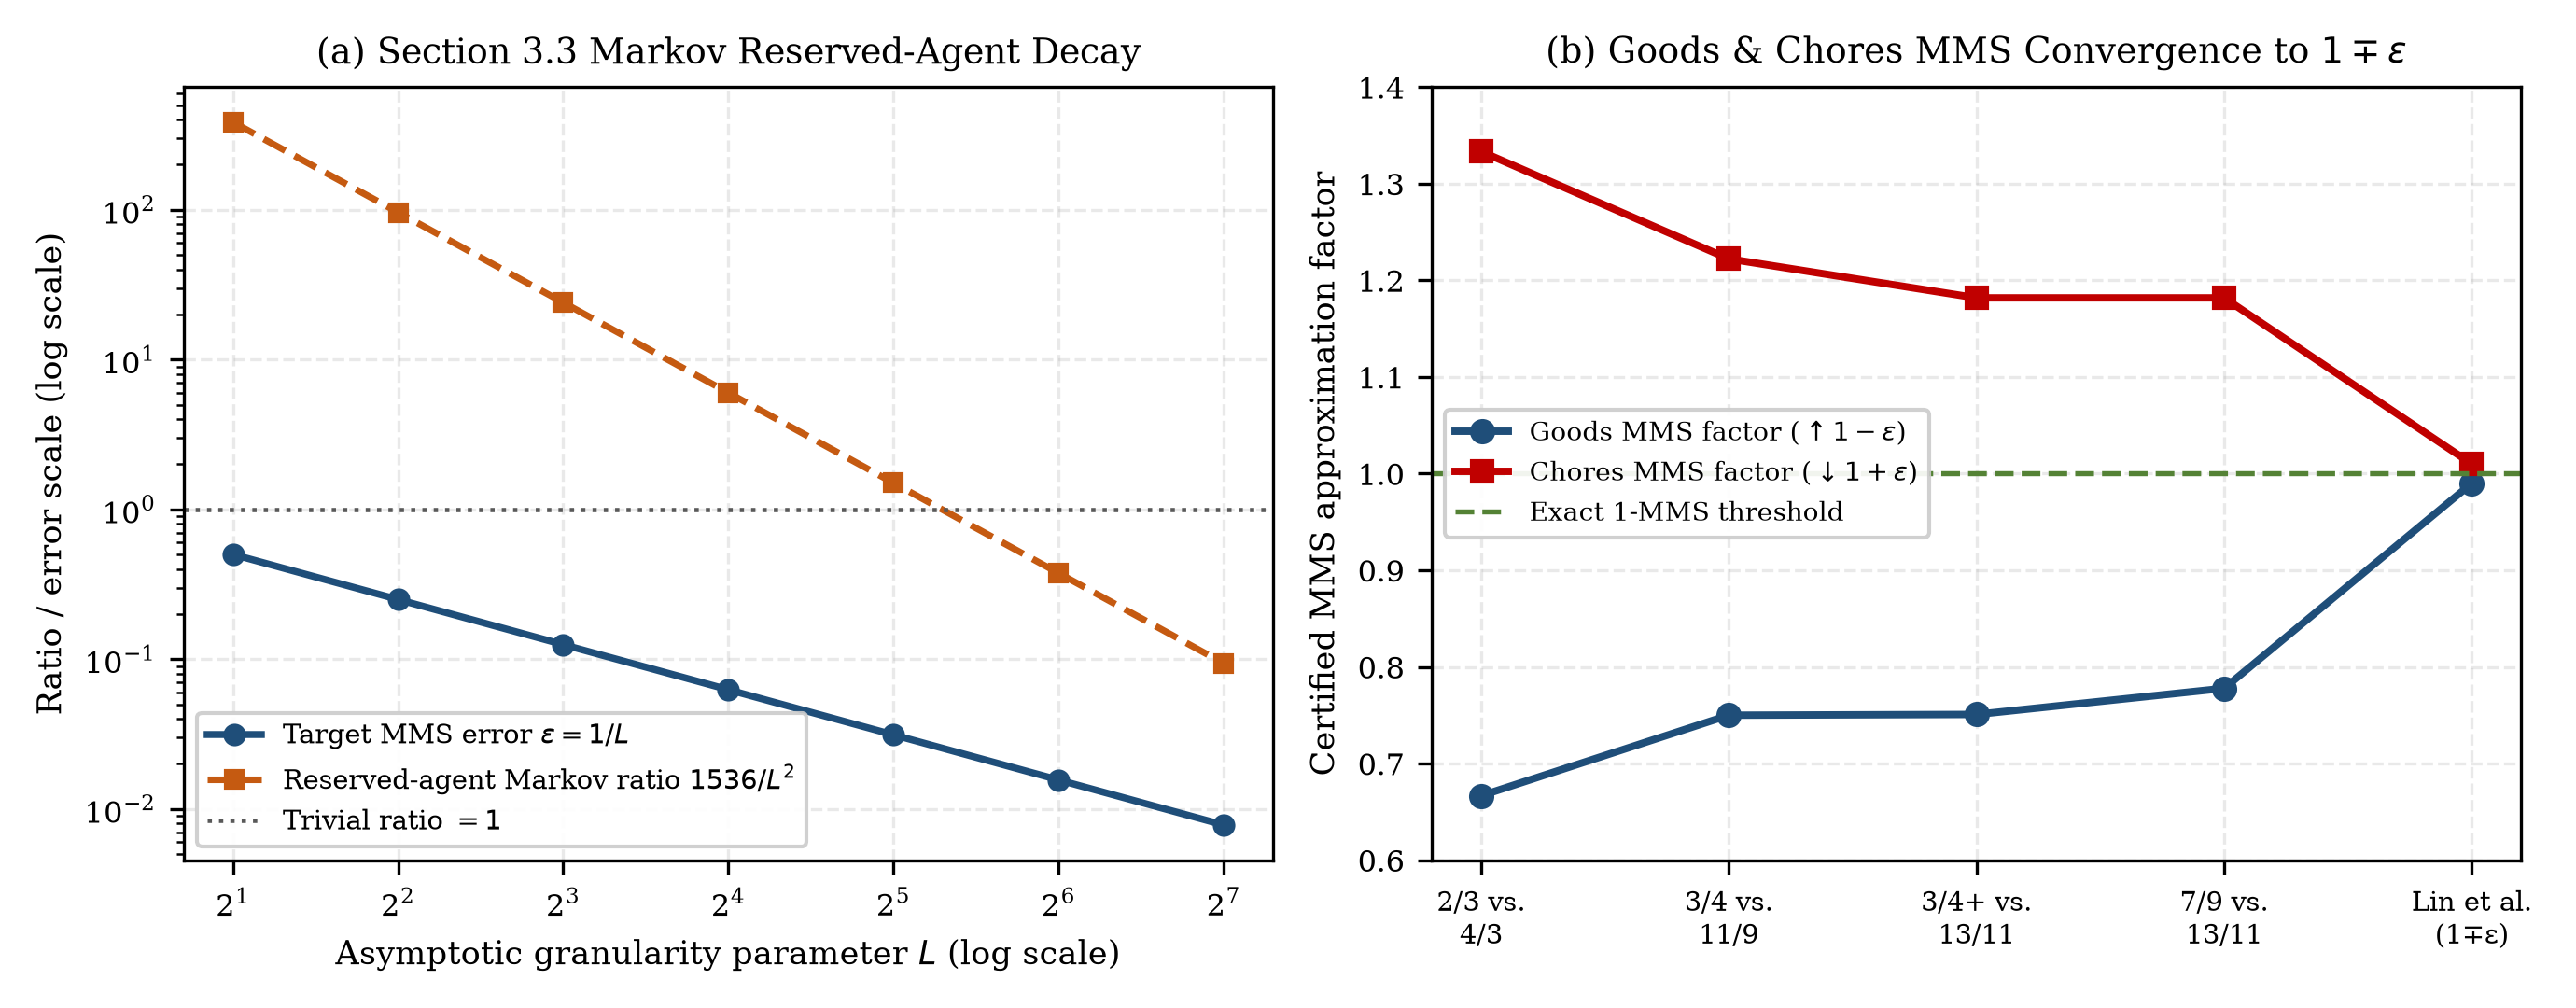
\includegraphics[width=\columnwidth]{../figures/fig2_markov_and_mms_landmarks.png}
  \caption{(a) Section~3.3 Markov reserved-agent ratio $1536/L^2$ vs.\ target MMS error $\varepsilon = 1/L$ across $L=2\dots 128$. (b) Historical progression of goods ($\uparrow 1-\varepsilon$) and chores ($\downarrow 1+\varepsilon$) MMS guarantees converging to exact $1$-MMS~\cite{lin2026mms}.}
  \label{fig:markov}
\end{figure}

\paragraph{Dual Markov Decay and Goods/Chores MMS Landmarks (Fig.~\ref{fig:markov}).}
Across $L = 2\dots 128$, the Definition~3.7 reserved-agent bound $1536/L^2$ crosses below $1$ at $L=64$ ($0.375$) and drops to $0.09375$ at $L=128$ as $\varepsilon = 1/L \to 0.00781$. Mode~3 ($0.293$--$0.864\,\mathrm{ms}$) certifies dual price spectra across $n \in \{3,4,5,6\}$, including both all-ordinary instances and non-empty reserved sets ($|N_r|=1$ at $n=4, 6$) with tail price sums $p(M_2)$ down to $1/8$. Mode~4 ($0.213$--$0.316\,\mathrm{ms}$) certifies exact tight-witness $(1-\varepsilon)$-MMS goods ($19/20$ and $13/10$) and $(1+\varepsilon)$-MMS chores ($21/20$ balanced and $11/10$ single-dominant-chore $\mu_i = 10 > \bar{c}_i = 8$) allocations together with $28$ ordinal bundle comparisons.

\begin{figure}[t]
  \centering
  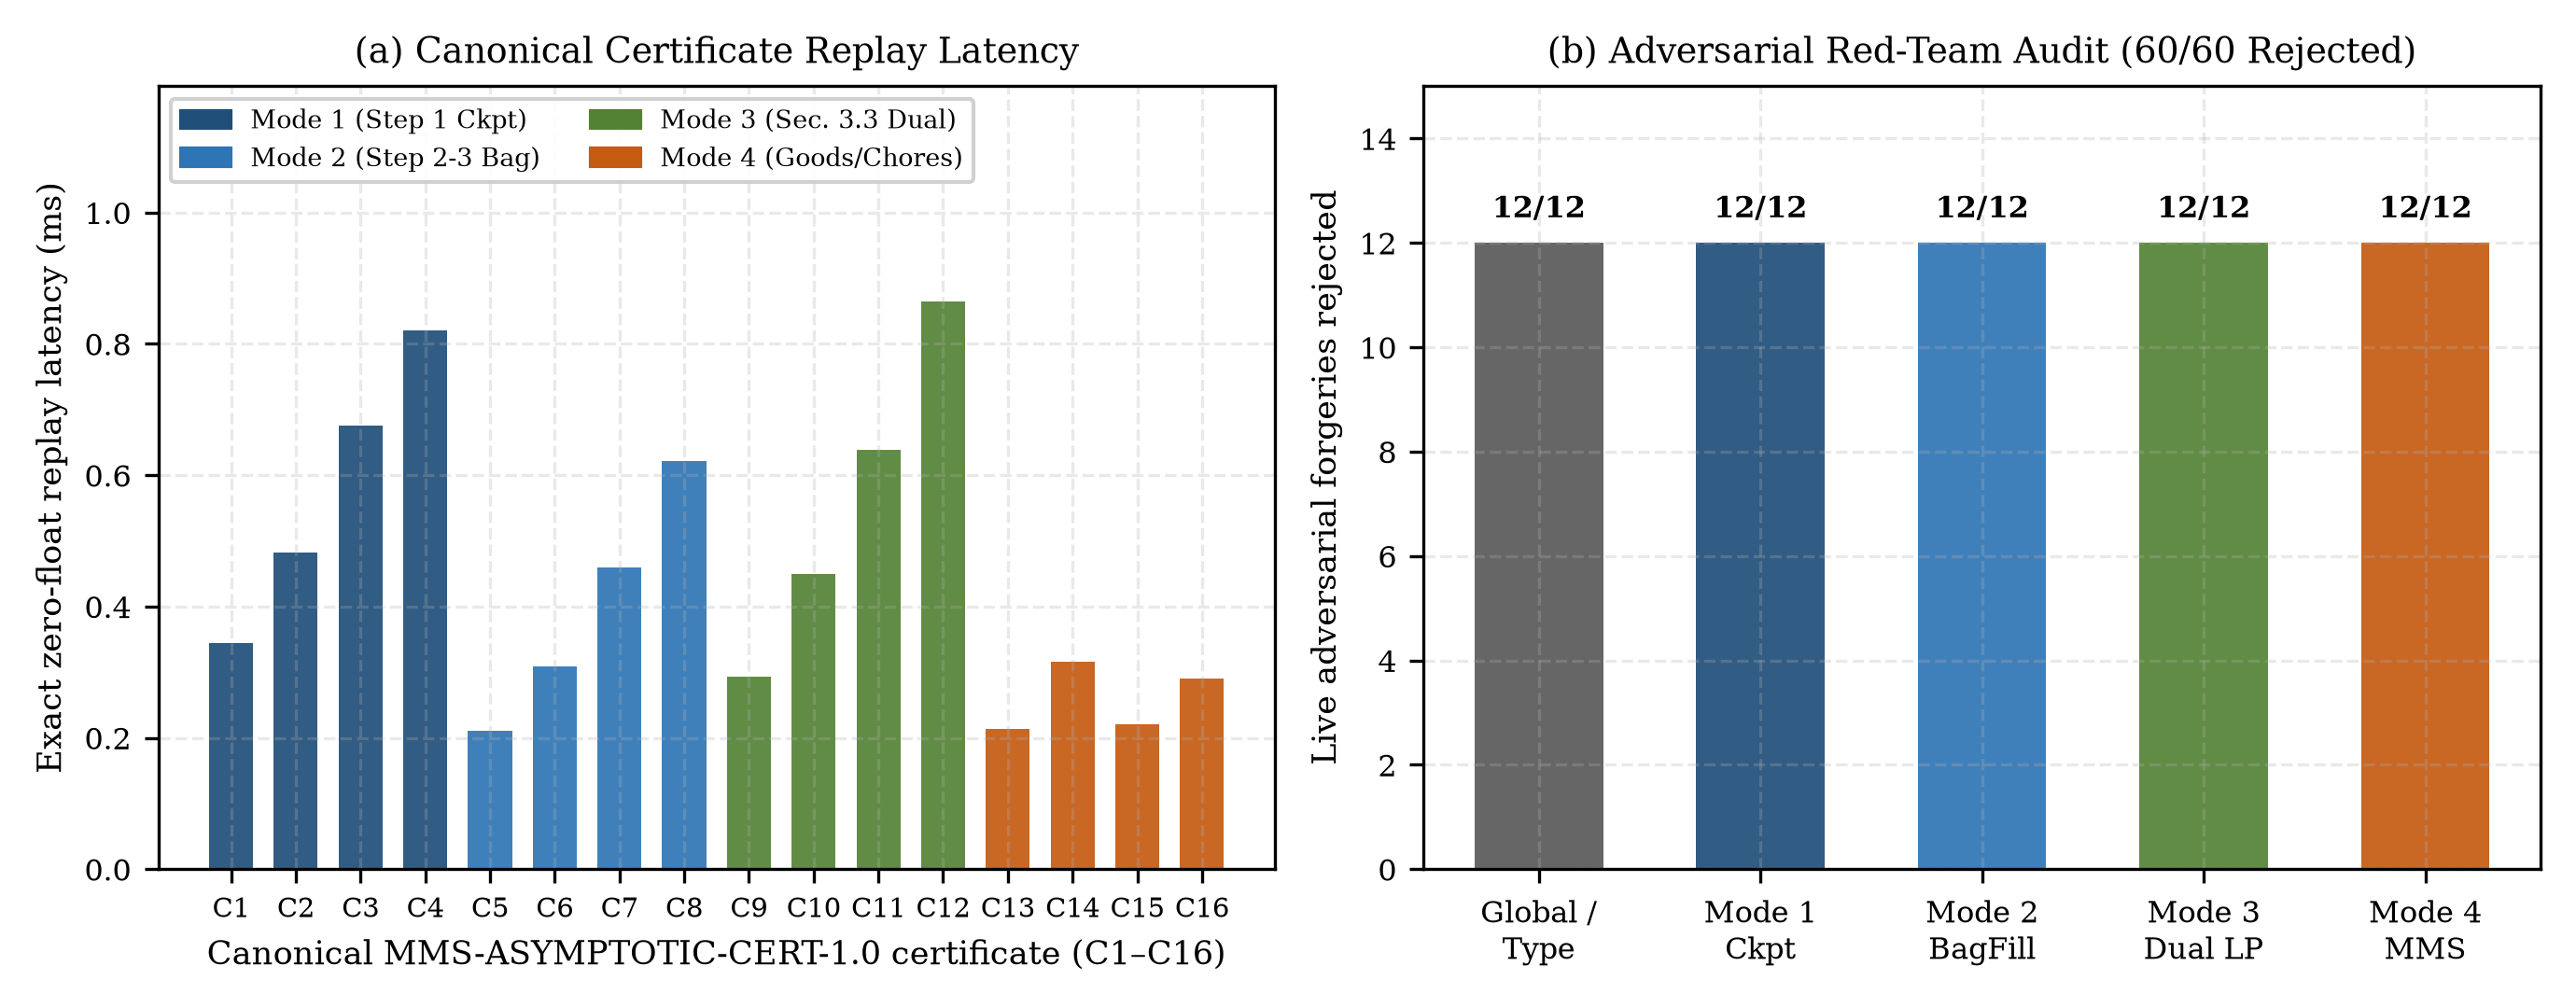
\includegraphics[width=\columnwidth]{../figures/fig3_certificate_replay_atlas.png}
  \caption{(a) Exact zero-float replay latency across all 16 canonical \texttt{MMS-ASYMPTOTIC-CERT-1.0} certificates ($0.211$--$0.864\,\mathrm{ms}$). (b) Red-team adversarial audit rejecting 60/60 live forgery attacks across five attack classes.}
  \label{fig:atlas}
\end{figure}

\paragraph{Replay Atlas and Red-Team Audit (Fig.~\ref{fig:atlas}, Table~\ref{tab:replay}).}
All 16 canonical certificates replay in $0.211$--$0.864\,\mathrm{ms}$ with zero floats. Our adversarial test suite (\texttt{tests/test\_suite.py}) executes 60 live forgery attacks—covering float/\texttt{None}/bool leaks, unreduced fractions, DoS bit-length caps, IDO and checkpoint-conservation violations, Step~2 deadline overflows, Step~3 starvation, dual-price and reduced-MMS violations, weak-witness MMS forgeries for both goods and chores, and forged ordinal queries—achieving \textbf{60/60 rejections} with zero bypasses.

\begin{table}[t]
\centering
\caption{Summary of all 16 canonical \texttt{MMS-ASYMPTOTIC-CERT-1.0} certificates and 60/60 live adversarial red-team audit.}
\label{tab:replay}
\resizebox{\columnwidth}{!}{%
\begin{tabular}{@{}lccc@{}}
\toprule
Verification Mode & Certs & Latency (ms) & Attacks Rejected \\
\midrule
Mode~1: Step~1 Checkpoint Rounding & 4 & $0.345$--$0.820$ & 12/12 \\
Mode~2: Steps~2--3 Deadline \& BagFill & 4 & $0.211$--$0.621$ & 12/12 \\
Mode~3: Sec.~3.3 Dual LP \& Markov & 4 & $0.293$--$0.864$ & 12/12 \\
Mode~4: Goods/Chores $(1\mp\varepsilon)$-MMS & 4 & $0.213$--$0.316$ & 12/12 \\
Global Schema / Type / Rational & -- & -- & 12/12 \\
\midrule
\textbf{Total} & \textbf{16} & \textbf{0.211--0.864} & \textbf{60/60} \\
\bottomrule
\end{tabular}}
\end{table}

\section{Conclusion}
We delivered an 18-theorem zero-dependency Lean~4 kernel (0~\texttt{sorry}, 0~warnings, 0~\texttt{Classical.choice}) and the exact-$\QQ$ verifier \texttt{MMS-ASYMPTOTIC-CERT-1.0} for the checkpoint-rounding, deadline-slot, Abel-summation, dual-price Markov, and goods/chores allocation core of Lin et al.~\cite{lin2026mms}. Formalizing the full randomized subsampling and recursive small-slack induction for arbitrary $n \ge n_0(\varepsilon)$ in Lean~4 remains an exciting frontier for verified fair division.

\bibliographystyle{plain}
\bibliography{references}
\end{document}
